% SIAM Article Template
\documentclass[review,hidelinks,onefignum,onetabnum]{siamart220329}

% Information that is shared between the article and the supplement
% (title and author information, macros, packages, etc.) goes into
% ex_shared.tex. If there is no supplement, this file can be included
% directly.

% SIAM Shared Information Template
% This is information that is shared between the main document and any
% supplement. If no supplement is required, then this information can
% be included directly in the main document.


% Packages and macros go here
\usepackage{lipsum}
\usepackage{amsfonts}
\usepackage{graphicx}
\usepackage{epstopdf}
\usepackage{algorithmic}
\ifpdf
  \DeclareGraphicsExtensions{.eps,.pdf,.png,.jpg}
\else
  \DeclareGraphicsExtensions{.eps}
\fi

% Add a serial/Oxford comma by default.
\newcommand{\creflastconjunction}{, and~}

% Used for creating new theorem and remark environments
\newsiamremark{remark}{Remark}
\newsiamremark{hypothesis}{Hypothesis}
\crefname{hypothesis}{Hypothesis}{Hypotheses}
\newsiamthm{claim}{Claim}

% Sets running headers as well as PDF title and authors
\headers{A second order numerical methods for Reisz-Fractional Elliptic Equation on graded mesh }{Jianxing Han and Minghua Chen}

% Title. If the supplement option is on, then "Supplementary Material"
% is automatically inserted before the title.
\title{second-order error analysis for Fractional Laplacian via Riesz Derivatives on graded meshes\thanks{Submitted to the editors DATE.
}}

% Authors: full names plus addresses.
\author{Jianxing Han\thanks{School of Mathematics and Statistics, Lanzhou University, Lanzhou 730000, PR China
  (\email{hanjx2023@mail.lzu.edu.cn}).}
  \and Minghua Chen\thanks{School of Mathematics and Statistics, Lanzhou University, Lanzhou 730000, PR China 
  (\email{chen@mail.lzu.edu.cn}).}
}

\usepackage{amsopn}
\DeclareMathOperator{\diag}{diag}


%%% Local Variables: 
%%% mode:latex
%%% TeX-master: "ex_article"
%%% End: 


% Optional PDF information
\ifpdf
\hypersetup{
  pdftitle={An Example Article},
  pdfauthor={D. Doe, P. T. Frank, and J. E. Smith}
}
\fi

% The next statement enables references to information in the
% supplement. See the xr-hyperref package for details.

\externaldocument[][nocite]{ex_supplement}

% FundRef data to be entered by SIAM
%<funding-group specific-use="FundRef">
%<award-group>
%<funding-source>
%<named-content content-type="funder-name"> 
%</named-content> 
%<named-content content-type="funder-identifier"> 
%</named-content>
%</funding-source>
%<award-id> </award-id>
%</award-group>
%</funding-group>

\begin{document}

\maketitle

% REQUIRED
\begin{abstract}
  \textcolor{gray}{
    This is an example SIAM \LaTeX\ article. This can be used as a
    template for new articles.  Abstracts must be able to stand alone
    and so cannot contain citations to the paper's references,
    equations, etc.  An abstract must consist of a single paragraph and
    be concise. Because of online formatting, abstracts must appear as
    plain as possible. Any equations should be inline.
  }
\end{abstract}

% REQUIRED
\begin{keywords}
  example, \LaTeX
\end{keywords}

% REQUIRED
\begin{MSCcodes}
  68Q25, 68R10, 68U05
\end{MSCcodes}

\section{Introduction}
\textcolor{gray}{
  The introduction introduces the context and summarizes the
  manuscript. It is importantly to clearly state the contributions of
  this piece of work.
}

For \(\Omega=(0,2T)\), \(1<\alpha<2\),
\textcolor{orange}{suppose \(f\in C^\beta(\Omega)\cap L^\infty(\Omega), \beta>4-\alpha, \|f\|_{\beta}^{\alpha/2}<\infty\)}
\begin{equation} \label{eq:equation}
  \begin{cases}
    (-\Delta)^{\frac{\alpha}{2}} u(x) = f(x), & x \in \Omega                      \\
    u(x) = 0,                                 & x \in \mathbb{R} \setminus \Omega
  \end{cases}
\end{equation}
where
\begin{equation} \label{def:operator}
  (-\Delta)^{\frac{\alpha}{2}} u(x) = -\frac{\partial^\alpha u}{\partial |x|^\alpha}
  = -\kappa_\alpha \frac{d^2}{dx^2} \int_\Omega \frac{|x-y|^{1-\alpha}}{\Gamma(2-\alpha)}u(y) dy
\end{equation}
\begin{equation} \label{def:kappa}
  \kappa_\alpha = -\frac{1}{2\cos(\alpha\pi/2)} > 0
\end{equation}

\section{Regularity}
\label{sec:regularity}

\textcolor{pink}{
  \begin{remark}
    1. \(C^k(U)\) is the set of all \(k\)-times continuously differentiable functions on open set \(U\). \\
    2. \(C^\beta(U)\) is the collection of function \(f\)  which for any \(V\subset\subset U\) \(f|_V\in C^\beta(\bar{V})\).   \\
    % 3. The condition \(f\in L^\infty(\Omega)\) may be unessecary, but we have not proven it yet, the numerical examples is shown in \cref{sec:experiments}.
  \end{remark}
}

\textcolor{orange}{
  \begin{theorem} \label{thm:regularity-f}
    If \(f\in C^\beta(\Omega), \beta>2\) and \(\|f\|_{\beta}^{(\alpha/2)}<\infty\), then for \(l=0, 1, 2\)
    \begin{equation}
      |f^{(l)}(x)| \le \|f\|_{\beta}^{(\alpha/2)} \begin{cases}
        x^{-l-\alpha/2}, & \text{if } 0 < x \le T \\ (2T-x)^{-l-\alpha/2}, & \text{if } T\le x < 2T
      \end{cases}
    \end{equation}
  \end{theorem}
}

\textcolor{orange}{
  \begin{theorem}[Regularity up to the boundary \cite{ROSOTON2014275}] \label{thm:regularity}
    \begin{equation}
      \|u\|_{\beta+\alpha}^{(-\alpha/2)} \le C \left( \|u\|_{C^{\alpha/2}(\mathbb{R})} + \|f\|_{\beta}^{(\alpha/2)} \right)
    \end{equation}
  \end{theorem}
  \begin{corollary} \label{cor:regularity-u}
    Let $u$ be a solution of \eqref{eq:equation} on $\Omega$. Then, for any $x\in\Omega$ and \(l=0, 1, 2, 3, 4\)
    \begin{equation}
      |u^{(l)}(x)| \le C \begin{cases}
        x^{\alpha/2-l}, & \text{if } 0 < x \le T \\ (2T-x)^{\alpha/2-l}, & \text{if } T\le x < 2T
      \end{cases}
    \end{equation}
  \end{corollary}
}


% The outline is not required, but we show an example here.
\textcolor{gray}{
  The paper is organized as follows. Our main results are in
  \cref{sec:main},  experimental
  results are in \cref{sec:experiments}, and the conclusions follow in
  \cref{sec:conclusions}.
}

\section{Numeric Format}
\label{sec:numformat}


\begin{equation} \label{def:xj}
  x_i = \begin{cases}
    T \left(\frac{i}{N}\right)^r   ,      & 0 \le i \le N  \\
    2T - T \left(\frac{2N-i}{N}\right)^r, & N \le i \le 2N
  \end{cases}
\end{equation}
where $r\ge 1$ .
And let
\begin{equation} \label{def:hj}
  h_j = x_{j} - x_{j-1}, \quad 1\le j \le 2N
\end{equation}

Let $\{\phi_j(x)\}_{j=1}^{2N-1}$ be standard hat functions, which are basis of the piecewise linear function space.
\begin{equation}
  \phi_j(x) = \begin{cases}
    \frac{1}{h_j} (x-x_{j-1}),      & x_{j-1} \le x \le x_{j} \\
    \frac{1}{h_{j+1}} (x_{j+1}-x) , & x_{j} \le x \le x_{j+1} \\
    0,                              & \text{otherwise}
  \end{cases}
\end{equation}
And then, we can approximate $u(x)$ with
\begin{equation}
  u_h(x) := \sum_{j=1}^{2N-1} u(x_j) \phi_j(x)
\end{equation}

For convience, we denote
\begin{equation} \label{def:Ih}
  I_h^{2-\alpha}(x_i) := \frac{1}{\Gamma(2-\alpha)}\int_{\Omega} |x_i-y|^{1-\alpha} u_h(y) dy
\end{equation}
And now, we can approximate the operator \eqref{def:operator} at $x_i$ with
\begin{equation} \label{def:Dhalpha}
  \begin{aligned}
    D_h^{\alpha} u_h(x_i) & := D_h^2 I_h^{2-\alpha}(x_i) \\
                          & =\frac{2}{h_{i} + h_{i+1}}
    \left( \frac{1}{h_{i}} I_h^{2-\alpha}(x_{i-1}) - \left( \frac{1}{h_{i}} + \frac{1}{h_{i+1}} \right) I_h^{2-\alpha}(x_{i}) + \frac{1}{h_{i+1}} I_h^{2-\alpha}(x_{i+1}) \right)
  \end{aligned}
\end{equation}
Finally, we approximate the equation \eqref{eq:equation} with
\begin{equation} \label{def:discrete_equation}
  -\kappa_\alpha D_h^{\alpha} u_h(x_i) = f(x_i), \quad 1\le i \le 2N-1
\end{equation}


The discrete equation \eqref{def:discrete_equation} can be written in matrix form
\begin{equation} \label{eq:equation_matrix}
  AU = F
\end{equation}
where $U$ is unknown, $F=(f(x_1), \cdots, f(x_{2N-1}))$.
The matrix $A$ is constructed as follows:
Since
\begin{equation}
  \begin{aligned} \label{eq:Ih}
    I_h^{2-\alpha}(x_i) & = \frac{1}{\Gamma(2-\alpha)} \int_{\Omega} |x_i-y|^{1-\alpha} u_h(y) dy                                                                     \\
                        & = \sum_{j=1}^{2N-1} \frac{1}{\Gamma(2-\alpha)} \int_{\Omega} |x_i-y|^{1-\alpha} u(x_j) \phi_j(y) dy                                         \\
                        & = \sum_{j=1}^{2N-1} u(x_j)  \frac{1}{\Gamma(2-\alpha)} \int_{x_{j-1}}^{x_{j+1}} |x_i-y|^{1-\alpha} \phi_j(y) dy                             \\
                        & = \sum_{j=1}^{2N-1} \frac{u(x_j)}{\Gamma(4-\alpha)}
    \left( \frac{|x_{i}-x_{j-1}|^{3-\alpha}}{h_{j}} -\frac{h_{j} + h_{j+1}}{h_{j}h_{j+1}}|x_i-x_{j}|^{3-\alpha} +  \frac{|x_{i}-x_{j+1}|^{3-\alpha}}{h_{j+1}} \right) \\
                        & =: \sum_{j=1}^{2N-1} \tilde{a}_{ij} \; u(x_j), \quad 0 \le i \le 2N
  \end{aligned}
\end{equation}
Then, substitute in \eqref{def:Dhalpha}, we have
\begin{equation}
  -\kappa_\alpha  D_h^{\alpha} u_h(x_i) = \sum_{j=1}^{2N-1} a_{ij} \; u(x_j)
\end{equation}
where
\begin{equation} \label{mat:aij}
  a_{ij} = -\kappa_\alpha \frac{2}{h_{i} + h_{i+1}}
  \left( \frac{1}{h_{i}} \tilde{a}_{i-1,j} - \left( \frac{1}{h_{i}} + \frac{1}{h_{i+1}} \right) \tilde{a}_{i,j} +  \frac{1}{h_{i+1}} \tilde{a}_{i+1, j} \right)
\end{equation}


\section{Main results}
\label{sec:main}


Here we state our main results; the proof is
deferred to \cref{sec:proof-truncation-error} and \cref{sec:proof-convergence}.

\textcolor{blue}{
  Let's denote \(h=\frac{1}{N}\), we have
  \begin{theorem}[Truncation Error] \label{thm:truncation-error}
    If $f \in C^2(\Omega)$ and $\alpha\in(1,2)$, and $u(x)$ is a solution of the equation \eqref{eq:equation}, then there exists a constant
    $C_1, C_2=C_1(T,\alpha, r, \|f\|_{C^2(\Omega)}), C_2(T,\alpha, r, \|f\|_{C^2(\Omega)})$, such that
    the truncation error of the discrete format satisfies
    \begin{equation} \label{eq:truncation-error}
      \begin{aligned}
        | -\kappa_\alpha D_h^{\alpha} u_h(x_i) - f(x_i) |
        \le & C_1 ( h^{r\alpha/2+r}(x_i^{-1-\alpha}+(2T-x_i)^{-1-\alpha}) \\
            & + h^2(x_i^{-\alpha/2-2/r} + (2T-x_i)^{-\alpha/2-2/r}) )     \\
            & + C_2 h^2
        \begin{cases}
          |T-x_{i-1}|^{1-\alpha}, \quad 1\le i\le N \\
          |T-x_{i+1}|^{1-\alpha} , \quad N<i\le 2N-1
        \end{cases}
      \end{aligned}
    \end{equation}
    where \(C_2=0\) if \(r=1\).
  \end{theorem}
}


\textcolor{blue}{
  \begin{theorem}[Convergence]\label{thm:convergence}
    The discrete equation \eqref{def:discrete_equation} has sulotion $U$,
    and there exists a positive constant $C=C(T,\alpha, r, \|f\|_{C^2(\Omega)})$
    such that the error between the numerial solution $U$ with the exact solution $u(x_i)$ satisfies
    \begin{equation} \label{eq:error}
      \max_{1\le i \le 2N-1} |U_i - u(x_i)| \le C h^{\min\{\frac{r\alpha}{2}, 2\}}
    \end{equation}
    That means the numerial method has convergence order ${\min\{\frac{r\alpha}{2}, 2\}}$.
  \end{theorem}
}



\section{Proof of \cref{thm:truncation-error}}
\label{sec:proof-truncation-error}

For convience, let's denote
\begin{equation}
  I^{2-\alpha}(x) = \frac{1}{\Gamma(2-\alpha)} \int_{\Omega} |x-y|^{1-\alpha} u(y) dy
\end{equation}
Then, the truncation error of the discrete format can be written as
\begin{equation} \label{eq:truncerrordepart}
  \begin{aligned}
    - \kappa_\alpha D_h^{\alpha} u_h(x_i) - f(x_i)
     & = -\kappa_\alpha (D_h^2 I_h^{2-\alpha}(x_i) - \frac{d^2}{dx^2} I^{2-\alpha}(x_i))                                           \\
     & = -\kappa_\alpha D_h^2 (I_h^{2-\alpha}-I^{2-\alpha})(x_i) - \kappa_\alpha (D_h^2 - \frac{d^2}{dx^2}) I^{2-\alpha}(x_i) \\
  \end{aligned}
\end{equation}


\subsection{Estimate of $-\kappa_\alpha (D_h^2 - \frac{d^2}{dx^2}) I^{2-\alpha} (x_i)$}

\textcolor{blue}{
  \begin{theorem} \label{lmm:trunerror2}
    There exits a constant $C=C(T,\alpha, r, \|f\|_{\beta}^{(\alpha/2)})$ such that
    \begin{equation}
      \left|-\kappa_\alpha (D_h^2 - \frac{d^2}{dx^2}) I^{2-\alpha} (x_i) \right| \le C h^2 (x_i^{-\alpha/2-2/r} + (2T-x_i)^{-\alpha/2-2/r})
    \end{equation}
  \end{theorem}
  \begin{proof}
    Since \(f\in C^2(\Omega)\) and
    \begin{equation}
      \frac{d^2}{dx^2} ( - \kappa_\alpha I^{2-\alpha}(x)) = f(x),  \quad x \in \Omega,
    \end{equation}
    we have \(I^{2-\alpha} \in C^4(\Omega)\).
    Therefore, using equation \eqref{eq:Dh2simd4} of \cref{lmm:Dh2simd2}, for \(1\le i\le 2N-1\), we have
    \begin{equation}
      \begin{aligned}
        -\kappa_\alpha (D_h^2 - \frac{d^2}{dx^2}) I^{2-\alpha} (x_i)
         & = \frac{h_{i+1}-h_{i}}{3} f'(x_i) + \frac{1}{4!} \frac{2}{h_i + h_{i+1}}(h_i^3 f''(\eta_1) + h_{i+1}^3 f''(\eta_2)) \\
      \end{aligned}
    \end{equation}
    where \(\eta_1 \in [x_{i-1}, x_{i}], \eta_2 \in [x_{i}, x_{i+1}]\).
    By \cref{lmm:hi1-hi} and \cref{thm:regularity-f}  we have
    1.
    \begin{equation}
      \left| \frac{h_{i+1}-h_{i}}{3} f'(x_i) \right| \le \frac{\|f\|_{\beta}^{(\alpha/2)}}{3} C h^2 \begin{cases}
        x_i^{-\alpha/2-2/r} ,     & 1\le i\le N-1 \\
        0,                        & i=N           \\
        (2T-x_i)^{-\alpha/2-2/r}, & N<i\le 2N-1
      \end{cases}
    \end{equation}
    2.
    See \cref{prf:trucerr2d2f}, there is a constant \(C=C(T, \alpha, r, \|f\|_{\beta}^{\alpha/2})\) such that
    \begin{equation}
      \begin{aligned}
         & \left| \frac{1}{4!} \frac{2}{h_i + h_{i+1}} (h_i^3 f''(\eta_1) + h_{i+1}^3 f''(\eta_2)) \right| \\
         & \quad \le C h^2 \begin{cases}
                             x_i^{-\alpha/2-2/r} ,     & 1\le i\le N    \\
                             (2T-x_i)^{-\alpha/2-2/r}, & N\le i\le 2N-1
                           \end{cases}
      \end{aligned}
    \end{equation}
    Summarizes, we get the result.
  \end{proof}
}


\subsection{Estimate of $R_i$}
\label{subsec:Ri}

Now, we study the first part of \cref{eq:truncerrordepart}
\begin{equation}
  \begin{aligned}
    D_h^2(I^{2-\alpha}-I_h^{2-\alpha})(x_i)
     & = D_h^2(\int_{0}^{2T}(u(y)-u_h(y)) \frac{|y-x_i|^{1-\alpha}}{\Gamma(2-\alpha)} dy) \\
  \end{aligned}
\end{equation}
For convience, let's denote
\begin{equation} \label{def:Tij}
  T_{ij} = \int_{x_{j-1}}^{x_{j}} (u(y) - u_h(y)) \frac{|y-x_i|^{1-\alpha}}{\Gamma(2-\alpha)} dy
\end{equation}
And define
\begin{equation} \label{eq:Ri}
  \begin{aligned}
    R_i &:= D_h^2(I^{2-\alpha}- I_h^{2-\alpha})(x_i) \\
    &= \frac{2}{h_{i} + h_{i+1}}  \sum_{j=1}^{2N}  \left( \frac{1}{h_{i}}  T_{i-1,j} - \left(\frac{1}{h_{i}} + \frac{1}{h_{i+1}}\right)  T_{i,j} + \frac{1}{h_{i+1}} T_{i+1,j} \right)
  \end{aligned}
\end{equation}


We have some results about the estimate of $R_i$

\begin{theorem} \label{Ri-ilessNdiv2}
  For \(1\le i < N/2\), there exists a constant $C$ such that
  \begin{equation}
    R_i \le C ( h^{r\alpha/2+r}x_i^{-1-\alpha} + h^2 x_i^{-\alpha/2-2/r} )
  \end{equation}
\end{theorem}

\textcolor{orange}{
\begin{theorem} \label{Ri-igreaterNdiv2-2}
  For \(N/2 \le i\le N\), there exists constant $C, C_2$ such that
  \begin{equation}
    R_i \le C h^2 x_i^{-\alpha/2-2/r} + C_2 h^2 |T-x_{i-1}|^{1-\alpha}
  \end{equation}
  where \(C_2=0\) if \(r=1\).
\end{theorem}
}

And for \(N<i\le 2N-1\), it is symmetric to the previous case.

To prove these results, we need some utils.
Also for simplicity, we denote
\begin{equation}
  S_{ij} =  \frac{2}{h_{i} + h_{i+1}}  \left( \frac{1}{h_{i}}  T_{i-1,j} - \left(\frac{1}{h_{i}} + \frac{1}{h_{i+1}}\right)  T_{i,j} + \frac{1}{h_{i+1}} T_{i+1,j} \right)
\end{equation}
then
\begin{equation}
  R_i = \sum_{j=1}^{2N} S_{ij}
\end{equation}

\begin{lemma} \label{lmm:Ti1}
  While \(0 \le i < N/2\),
  By \cref{lmm:Dyj1}
  \begin{equation}
    \begin{aligned}
      |T_{i1}| &\le C \int_{0}^{x_1} x_1^{\alpha/2} \frac{|x_i-y|^{1-\alpha}}{\Gamma(2-\alpha)} dy \\
      &= C \frac{1}{\Gamma(3-\alpha)} x_1^{\alpha/2}  \left| x_i^{2-\alpha} - |x_i-x_1|^{2-\alpha} \right| \\
      &\le C \frac{1}{\Gamma(3-\alpha)} x_1^{\alpha/2 + 2-\alpha} =  C \frac{1}{\Gamma(3-\alpha)} x_1^{2-\alpha/2} \quad 0<2-\alpha<1
    \end{aligned}
  \end{equation}
  For \(2\le j \le N\), by \cref{lmm:Dyj}
  \begin{equation}
    \begin{aligned}
      |T_{ij}| &\le \frac{C}{4} \int_{x_{j-1}}^{x_j} h_j^2 x_{j-1}^{\alpha/2-2}  \frac{|y-x_i|^{1-\alpha}}{\Gamma(2-\alpha)} dy \\
      & \le \frac{C}{4 \Gamma(3-\alpha)}  h_j^2 x_{j-1}^{\alpha/2-2}  \left| |x_j-x_i|^{2-\alpha} - |x_{j-1}-x_{i}|^{2-\alpha} \right| \\
    \end{aligned}
  \end{equation}
\end{lemma}

\textcolor{blue}{
\begin{lemma} \label{lmm:sumSi-ilessNdiv2-2ip1-N}
  While \(1 \le i < N/2\),
  \begin{equation}
    \begin{aligned}
      \sum_{j=\max\{2i+1, i+3\}}^{N} S_{ij} \le C h^2 x_i^{-\alpha/2-2/r}
    \end{aligned}
  \end{equation}
\end{lemma}
\begin{proof}
  For  \(\max\{2i+1, i+3\} \le j \le N\), by \cref{lmm:Dyjleh2yadiv2m2divr} and \cref{lmm:Dh2ymx1malecy1ma}
  \begin{equation}
    \begin{aligned}
      S_{ij} &= \int_{x_{j-1}}^{x_{j}}(u(y) - u_h(y)) D_h^2 \left(\frac{|y-\cdot|^{1-\alpha}}{\Gamma(2-\alpha)}\right)(x_i) dy \\
      % &\le C h^2 \int_{x_{j-1}}^{x_{j}} y^{\alpha/2-2/r} \frac{|y-x_{i+1}|^{-1-\alpha}}{\Gamma(-\alpha)} dy \\
      &\le C h^2 \int_{x_{j-1}}^{x_{j}} y^{\alpha/2-2/r} \frac{y^{-1-\alpha}}{\Gamma(-\alpha)} dy   \\
      &= C h^2 \int_{x_{j-1}}^{x_{j}} y^{-\alpha/2-2/r-1} dy
    \end{aligned}
  \end{equation}
  Therefore,
  \begin{equation}
    \begin{aligned}
      \sum_{j=\max\{2i+1, i+3\}}^{N} S_{ij} &\le C h^2 \int_{x_{2i}}^{x_{N}} y^{-\alpha/2-2/r-1} dy \\
      &= \frac{C}{\alpha/2+2/r} h^2 ( 2^{r(-\alpha/2-2/r)} x_i^{-\alpha/2-2/r} - T^{-\alpha/2-2/r})
    \end{aligned}
  \end{equation}
\end{proof}
}

\section{Proof of \cref{thm:convergence}}
\label{sec:proof-convergence}

\section{Experimental results}
\label{sec:experiments}

% \textcolor{gray}{
%   \Cref{fig:testfig} shows some example results. Additional results are
%   available in the supplement in \cref{tab:foo}.
%   \begin{figure}[htbp]
%     \centering
%     \label{fig:a}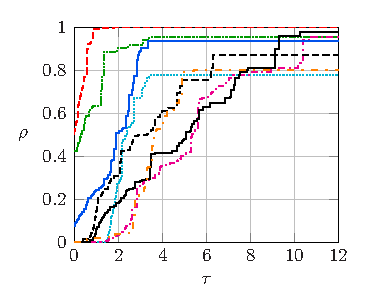
\includegraphics{lexample_fig1}
%     \caption{Example figure using external image files.}
%     \label{fig:testfig}
%   \end{figure}
%   \Cref{tab:foo} shows additional
%   supporting evidence.
% }
% \textcolor{gray}{
%   \begin{table}[htbp]
%     \footnotesize
%     \caption{Example table.}\label{tab:foo}
%     \begin{center}
%       \begin{tabular}{|c|c|c|} \hline
%         Species & \bf Mean & \bf Std.~Dev. \\ \hline
%         1       & 3.4      & 1.2           \\
%         2       & 5.4      & 0.6           \\
%         3       & 7.4      & 2.4           \\
%         4       & 9.4      & 1.8           \\ \hline
%       \end{tabular}
%     \end{center}
%   \end{table}
% }

% \section{Discussion of \texorpdfstring{{\boldmath$Z=X \cup Y$}}{Z = X union Y}}


\section{Conclusions}
\label{sec:conclusions}

Some conclusions here.


\appendix

\section{Approximate of difference quotients}

\begin{lemma} \label{lmm:Dh2simd2}
  If \(g(x)\) is twice differentable continous function on open set $\Omega$,
  there exists \(\xi \in [x_{i-1}, x_{i+1}]\) such that
  \begin{equation} \label{eq:Dh2simd2}
    \begin{aligned}
      D_h^2 g(x_i) &:= \frac{2}{h_i + h_{i+1}} \left( \frac{1}{h_{i+1}} g(x_{i+1}) - (\frac{1}{h_{i}}+\frac{1}{h_{i+1}})g(x_{i}) + \frac{1}{h_{i}} g(x_{i-1}) \right) \\
      % &= \frac{h_i}{h_i + h_{i+1}} g''(\xi_1) + \frac{h_{i+1}}{h_i + h_{i+1}} g''(\xi_2)  \\
                              & = g''(\xi), \quad \xi \in [x_{i-1}, x_{i+1}]
    \end{aligned}
  \end{equation}
  \begin{equation} \label{eq:Dh2Cauchy2}
    \begin{aligned}
       & \frac{2}{h_i + h_{i+1}} \left( \frac{1}{h_{i+1}} g(x_{i+1}) - (\frac{1}{h_{i}}+\frac{1}{h_{i+1}})g(x_{i}) + \frac{1}{h_{i}} g(x_{i-1}) \right)                          \\
      % &= \frac{h_i}{h_i + h_{i+1}} g''(\xi_1) + \frac{h_{i+1}}{h_i + h_{i+1}} g''(\xi_2)  \\
       & \quad = \frac{2}{h_i + h_{i+1}} \left( \frac{1}{h_{i}}\int_{x_{i-1}}^{x_i} g''(y) (y-x_{i-1}) dy + \frac{1}{h_{i+1}} \int_{x_i}^{x_{i+1}} g''(y) (x_{i+1}-y) dy \right)
    \end{aligned}
  \end{equation}
  And if \(g(x) \in C^4(\Omega)\), then
  \begin{equation} \label{eq:Dh2simd4}
    \begin{aligned}
      \frac{2}{h_i + h_{i+1}} & \left( \frac{1}{h_{i+1}} g(x_{i+1}) - (\frac{1}{h_{i}}+\frac{1}{h_{i+1}})g(x_{i}) + \frac{1}{h_{i}} g(x_{i-1}) \right)                   \\
                              & = g''(x_{i}) + \frac{h_{i+1}-h_{i}}{3} g'''(x_{i}) + \frac{1}{4!} \frac{2}{h_i + h_{i+1}}(h_i^3 g''''(\eta_1) + h_{i+1}^3 g''''(\eta_2))
    \end{aligned}
  \end{equation}
  where \(\eta_1 \in [x_{i-1}, x_{i}], \eta_2 \in [x_{i}, x_{i+1}]\).
\end{lemma}
\begin{proof}
  \begin{gather*}
    g(x_{i-1}) = g(x_{i}) - (x_{i}-x_{i-1}) g'(x_{i}) + \frac{(x_{i}-x_{i-1})^2}{2} g''(\xi_1), \quad \xi_1 \in [x_{i-1}, x_{i}]        \\
    g(x_{i+1}) = g(x_{i}) + (x_{i+1}-x_{i}) g'(x_{i}) + \frac{(x_{i+1}-x_{i})^2}{2} g''(\xi_2), \quad \xi_2 \in [x_{i}, x_{i+1}]
  \end{gather*}
  Subsitute them in the left side of \eqref{eq:Dh2simd2}, we have
  \begin{equation*}
    \begin{aligned}
      \frac{2}{h_i + h_{i+1}} & \left( \frac{1}{h_{i+1}} g(x_{i+1}) - (\frac{1}{h_{i}}+\frac{1}{h_{i+1}})g(x_{i}) + \frac{1}{h_{i}} g(x_{i-1}) \right) \\
                              & = \frac{h_i}{h_i + h_{i+1}} g''(\xi_1) + \frac{h_{i+1}}{h_i + h_{i+1}} g''(\xi_2)
    \end{aligned}
  \end{equation*}
  Now, using intermediate value theorem , there exists \(\xi \in [\xi_1, \xi_2]\) such that
  \begin{equation*}
    \frac{h_i}{h_i + h_{i+1}} g''(\xi_1) + \frac{h_{i+1}}{h_i + h_{i+1}} g''(\xi_2) = g''(\xi)
  \end{equation*}
  For the second equation, similarly
  \begin{gather*}
    g(x_{i-1}) = g(x_{i}) - (x_{i}-x_{i-1}) g'(x_{i}) + \int_{x_{i-1}}^{x_i} g''(y) (y-x_{i-1}) dy \\
    g(x_{i+1}) = g(x_{i}) + (x_{i+1}-x_{i}) g'(x_{i}) + \int_{x_i}^{x_{i+1}} g''(y) (x_{i+1}-y) dy
  \end{gather*}
  And the last equation can be obtained by
  \begin{gather*}
    g(x_{i-1}) = g(x_{i}) - h_{i} g'(x_{i}) + \frac{h_{i}^2}{2} g''(x_{i}) - \frac{h_{i}^3}{3!} g'''(x_{i}) +  \frac{h_{i}^4}{4!} g''''(\eta_1)         \\
    g(x_{i+1}) = g(x_{i}) + h_{i+1} g'(x_{i}) + \frac{h_{i+1}^2}{2} g''(x_{i}) + \frac{h_{i+1}^3}{3!} g'''(x_{i}) + \frac{h_{i+1}^4}{4!} g''''(\eta_2)
  \end{gather*}
  where \(\eta_1 \in [x_{i-1}, x_{i}], \eta_2 \in [x_{i}, x_{i+1}]\).
  Expecially,
  \begin{equation} \label{eq:Dh2Cauchy4}
    \begin{aligned}
      \frac{h_i^4}{4!}g''''(\eta_1)     & = \int_{x_{i-1}}^{x_{i}} g''''(y) \frac{(y-x_{i-1})^3}{3!} dy \\
      \frac{h_{i+1}^4}{4!}g''''(\eta_2) & = \int_{x_{i}}^{x_{i+1}} g''''(y) \frac{(x_{i+1}-y)^3}{3!} dy
    \end{aligned}
  \end{equation}
  Subsitute them to the left side of \eqref{eq:Dh2simd4}, we can get the result.
\end{proof}


\begin{lemma} \label{lmm:Dyj}
  If \(y\in [x_{j-1}, x_j]\), denote \(y = \theta x_{j-1} + (1-\theta) x_j, \theta\in [0,1]\),
  % then for \(2\le j \le 2N-1\)
  \begin{equation}
    \begin{aligned}
      u(y_j^\theta) - u_h(y_j^\theta) & = -\frac{\theta (1-\theta)}{2} h_j^2 u''(\xi), \quad \xi \in [x_{j-1}, x_j]
    \end{aligned}
  \end{equation}
  \begin{equation}
    \begin{aligned}
      u(y_j^\theta) - u_h(y_j^\theta) = & -\frac{\theta (1-\theta)}{2} h_j^2 u''(y_j^\theta)
      + \frac{\theta (1-\theta)}{3!} h_j^3 (\theta^2 u'''(\eta_1) - (1-\theta)^2 u'''(\eta_2))
    \end{aligned}
  \end{equation}
  where \(\eta_1 \in [x_{j-1}, y_j^\theta], \eta_2 \in [y_j^\theta, x_j]\).
\end{lemma}
\begin{proof}
  By Taylor expansion, we have
  \begin{gather*}
    u(x_{j-1}) = u(y_j^\theta) - \theta h_{j} u'(y_j^\theta) + \frac{\theta^2 h_{j}^2}{2!} u''(\xi_1), \quad \xi_1 \in [x_{j-1}, y_j^\theta] \\
    u(x_{j}) = u(y_j^\theta) + (1-\theta) h_{j} u'(y_j^\theta) + \frac{(1-\theta)^2 h_{j}^2}{2!} u''(\xi_2) , \quad \xi_2 \in [y_j^\theta, x_j]
  \end{gather*}
  Thus
  \begin{equation*}
    \begin{aligned}
      u(y_j^\theta) - u_h(y_j^\theta) & = u(y_j^\theta) - (1-\theta)u(x_{j-1}) - \theta u(x_{j})                          \\
                                      & = -\frac{\theta (1-\theta)}{2} h_j^2 (\theta u''(\xi_1) + (1-\theta) u''(\xi_2) ) \\
                                      & = -\frac{\theta (1-\theta)}{2} h_j^2 u''(\xi), \quad \xi \in [\xi_1, \xi_2]
    \end{aligned}
  \end{equation*}
  The second equation is similar,
  \begin{gather*}
    u(x_{j-1}) = u(y_j^\theta) - \theta h_{j} u'(y_j^\theta) + \frac{\theta^2 h_{j}^2}{2!} u''(y_j^\theta) - \frac{\theta^3 h_{j}^3}{3!} u'''(\eta_1)  \\
    u(x_{j}) = u(y_j^\theta) + (1-\theta) h_{j} u'(y_j^\theta) + \frac{(1-\theta)^2 h_{j}^2}{2!} u''(y_j^\theta) + \frac{(1-\theta)^3 h_{j}^3}{3!} u'''(\eta_2)
  \end{gather*}
  where \(\eta_1 \in [x_{j-1}, y_j^\theta], \eta_2 \in [y_j^\theta, x_j]\).
  Thus
  \begin{equation*}
    \begin{aligned}
      u(y_j^\theta) - u_h(y_j^\theta) & = u(y_j^\theta) - (1-\theta)u(x_{j-1}) - \theta u(x_{j})                                                                                      \\
                                      & = -\frac{\theta (1-\theta)}{2} h_j^2 u''(y_j^\theta) + \frac{\theta (1-\theta)}{3!} h_j^3 (\theta^2 u'''(\eta_1) - (1-\theta)^2 u'''(\eta_2))
    \end{aligned}
  \end{equation*}
\end{proof}

\begin{lemma} \label{lmm:Dyj1}
  For \(x\in [x_{j-1}, x_j]\)
  \begin{equation}
    \begin{aligned}
      |u(x) - u_h(x)| &= \left| \frac{x_{j}-x}{h_j} \int_{x_{j-1}}^x u'(y) dy - \frac{x-x_{j-1}}{h_j} \int_{x}^{x_{j}} u'(y) dy \right| \\
      &\le \int_{x_{j-1}}^{x_{j}} |u'(y)| dy 
    \end{aligned}
  \end{equation}
  If \(x\in [0, x_1]\), with \cref{cor:regularity-u}, we have
  \begin{equation}
    |u(x) - u_h(x)| \le \int_{0}^{x_1} |u'(y)| dy \le \int_{0}^{x_1} C y^{\alpha/2-1} dy  \le C\frac{2}{\alpha} x_1^{\alpha/2}
  \end{equation}
  Similarly, if \(x\in [x_{2N-1}, 1]\), we have
  \begin{equation}
    |u(x) - u_h(x)| \le C\frac{2}{\alpha} (2T-x_{2N-1})^{\alpha/2} = C\frac{2}{\alpha} x_1^{\alpha/2}
  \end{equation}
\end{lemma}


\section{Inequality}

\textcolor{blue}{
  \begin{lemma} \label{lmm:hilexi}
    \begin{equation}
      h_i \le r T^{1/r} h \begin{cases}
        x_i^{1-1/r},          & 1\le i \le N   \\
        (2T-x_{i-1})^{1-1/r}, & N < i \le 2N-1
      \end{cases}
    \end{equation}
  \end{lemma}
  \begin{proof}
    For \(1\le i \le N\),
    \begin{displaymath}
      \begin{aligned}
        h_i & = T \left( \left(\frac{i}{N}\right)^r - \left(\frac{i-1}{N}\right)^r \right)  \\
            & \le rT \frac{1}{N} \left(\frac{i}{N}\right)^{r-1} = r T^{1/r} h x_{i}^{1-1/r} \\
      \end{aligned}
    \end{displaymath}
    For \(N < i \le 2N-1\),
    \begin{displaymath}
      \begin{aligned}
        h_i & = T\left(  \left(\frac{2N-i+1}{N}\right)^r - \left(\frac{2N-i}{N}\right)^r \right)        \\
            & \le rT \frac{1}{N} \left(\frac{2N-i+1}{N}\right)^{r-1} = r T^{1/r} h (2T-x_{i-1})^{1-1/r} \\
      \end{aligned}
    \end{displaymath}
  \end{proof}
}


\textcolor{blue}{
  \begin{lemma} \label{lmm:hi1-hi}
    There is a constant \(C=2^{|r-2|}r(r-1)T^{2/r}\) such that for all \(i\in\{1,2,\cdots,2N-1\}\)
    \begin{equation}
      |h_{i+1} - h_{i}| \le C h^2 \begin{cases}
        x_i^{1-2/r} ,     & 1\le i\le N-1 \\
        0,                & i=N           \\
        (2T-x_i)^{1-2/r}, & N<i\le 2N-1   \\
      \end{cases}
    \end{equation}
  \end{lemma}
  \begin{proof}
    \begin{equation*}
      \begin{aligned}
        h_{i+1} - h_{i} =
        \begin{cases}
          T \left( \left(\frac{i+1}{N}\right)^r - 2\left(\frac{i}{N}\right)^r + \left(\frac{i-1}{N}\right)^r  \right) ,           & 1\le i\le N-1    \\
          0,                                                                                                                      & i=N              \\
          -T \left( \left(\frac{2N-i-1}{N}\right)^r - 2\left(\frac{2N-i}{N}\right)^r + \left(\frac{2N-i+1}{N}\right)^r  \right) , & N+1\le i\le 2N-1 \\
        \end{cases}
      \end{aligned}
    \end{equation*}
    % if \(r=2\), 
    % \begin{equation*}
    %   h_{i+1}-h_{i} = 2T N^{-2}, \quad 1-2/r=0
    % \end{equation*}
    For \(i=1\),
    \begin{equation*}
      \begin{aligned}
        h_2-h_1 & = T(2^{r}-2)\left(\frac{1}{N}\right)^r = (2^{r}-2)T^{2/r} h^2 x_1^{1-2/r}
      \end{aligned}
    \end{equation*}
    For \(2\le i\le N-1\),
    \begin{equation*}
      \begin{aligned}
        h_{i+1} - h_{i} & =  r(r-1) T \; N^{-2} \eta^{r-2}, \quad \eta \in [\frac{i-1}{N}, \frac{i+1}{N}]
      \end{aligned}
    \end{equation*}
    If \(r\in[1, 2]\),
    \begin{equation*}
      \begin{aligned}
        h_{i+1} - h_{i} & =  r(r-1) T \; N^{-2} \eta^{r-2}
        \le r(r-1) T \; h^2 \left( \frac{i-1}{N} \right)^{r-2}                         \\
                        & \le r(r-1) T \; h^2 2^{2-r} \left( \frac{i}{N} \right)^{r-2} \\
                        & = 2^{2-r} r(r-1) T^{2/r} h^2 x_i^{1-2/r}
      \end{aligned}
    \end{equation*}
    else if \(r>2\),
    \begin{equation*}
      \begin{aligned}
        h_{i+1} - h_{i} & =  r(r-1) T \; N^{-2} \eta^{r-2}
        \le r(r-1) T \; h^2 \left( \frac{i+1}{N} \right)^{r-2}                         \\
                        & \le r(r-1) T \; h^2 2^{r-2} \left( \frac{i}{N} \right)^{r-2} \\
                        & = 2^{r-2} r(r-1) T^{2/r} h^2 x_i^{1-2/r}
      \end{aligned}
    \end{equation*}
    Since
    \begin{equation*}
      2^r-2 \le 2^{|r-2|}r(r-1), \quad r\ge 1
    \end{equation*}
    we have
    \begin{equation*}
      h_{i+1} - h_{i} \le 2^{|r-2|}r(r-1)T^{2/r} h^2 x_i^{1-2/r},  \quad 1\le i\le N-1
    \end{equation*}
    For \(i=N\), \( h_{N+1}-h_{N} = 0\).
    For \(N<i\le 2N-1\), it's central symmetric to the first half of the proof, which is
    % \begin{equation*}
    %   \begin{aligned}
    %     h_{2N-1} - h_{2N} & =
    %       T(2^{r}-2)\left(\frac{1}{N}\right)^r = (2^{r}-2)T^{2/r} h^2 (2T-x_{2N-1})^{1-2/r}
    %   \end{aligned}
    % \end{equation*}
    % and
    \begin{equation*}
      h_{i}-h_{i+1} \le 2^{|r-2|}r(r-1)T^{2/r} h^2 (2T-x_{i})^{1-2/r}
    \end{equation*}
    Summarizes the inequalities, we can get
    \begin{equation}
      |h_{i+1} - h_{i}| \le 2^{|r-2|}r(r-1)T^{2/r} h^2 \begin{cases}
        x_i^{1-2/r} ,     & 1\le i\le N-1 \\
        0,                & i=N           \\
        (2T-x_i)^{1-2/r}, & N<i\le 2N-1
      \end{cases}
    \end{equation}
  \end{proof}
}




\section{Proofs of some technical details}

\begin{proof}[Additional proof of \cref{lmm:trunerror2}] \label{prf:trucerr2d2f}
  For \(2\le i \le N-1\),
  \begin{equation*}
    \begin{aligned}
      \frac{2}{h_i + h_{i+1}} & (h_i^3 f''(\eta_1) + h_{i+1}^3 f''(\eta_2))                                                \\
                              & \le C\frac{2}{h_i + h_{i+1}} (h_i^3 x_{i-1}^{-2-\alpha/2} + h_{i+1}^3 x_{i}^{-2-\alpha/2}) \\
                              & \le 2C (h_i^2 x_{i-1}^{-2-\alpha/2} + h_{i+1}^2 x_{i}^{-2-\alpha/2})
    \end{aligned}
  \end{equation*}
  Since \cref{lmm:hilexi}, we have
  \begin{gather*}
    h_i \le r T^{1/r} h x_{i}^{1-1/r}, \quad 1\le i\le N \\
    h_{i+1} \le r T^{1/r} h x_{i+1}^{1-1/r}, \quad 1\le i\le N-1
  \end{gather*}
  and
  \begin{gather*}
    x_{i-1}^{-2-\alpha/2} \le 2^{-r(-2-\alpha/2)} x_i^{-2-\alpha/2}  \quad 2\le i\le N-1 \\
    x_{i+1}^{1-1/r} \le 2^{r-1} x_i^{1-1/r} \quad 1\le i \le N-1
  \end{gather*}
  So there is a constant \(C=C(T, \alpha, r, \|f\|_{\beta}^{\alpha/2})\) such that
  \begin{equation*}
    \frac{2}{h_i + h_{i+1}} (h_i^3 f''(\eta_1) + h_{i+1}^3 f''(\eta_2)) \le C h^2 x_i^{-\alpha/2-2/r}, \quad 2\le i\le N-1
  \end{equation*}
  For \(i=1\), by \eqref{eq:Dh2Cauchy4}
  \begin{equation*}
    \begin{aligned}
       & \frac{1}{4!}\frac{2}{h_1 + h_{2}} (h_1^3 f''(\eta_1) + h_{2}^3 f''(\eta_2))                  \\
       & \quad =  \frac{2}{h_1 + h_{2}} \left( \frac{1}{h_1}\int_{0}^{x_1} f''(y) \frac{y^3}{3!} dy +
      \frac{1}{4!} h_2^3 f''(\eta_2) \right)                                                          \\
    \end{aligned}
  \end{equation*}
  We have proved above that
  \begin{equation*}
    \frac{2}{h_1 + h_{2}} h_2^3 f''(\eta_2) \le C h^2 x_1^{-\alpha/2-2/r}
  \end{equation*}
  and we can get
  \begin{equation*}
    \begin{aligned}
      \int_{0}^{x_1} f''(y) \frac{y^3}{3!} dy & \le C \frac{1}{3!}\int_{0}^{x_1} y^{1-\alpha/2} dy \\
                                              & = C\frac{1}{3!(2-\alpha/2)} x_1^{2-\alpha/2}       \\
    \end{aligned}
  \end{equation*}
  so
  \begin{equation*}
    \frac{2}{h_1 + h_{2}} \frac{1}{h_1}\int_{0}^{x_1} f''(y) \frac{y^3}{3!} dy = \frac{C 2^{1-r}}{3!(2-\alpha/2)}x_1^{-\alpha/2} = \frac{C 2^{1-r}}{3!(2-\alpha/2)} T^{2/r} h^2 x_1^{-\alpha/2-2/r}
  \end{equation*}
  And for \(i=N\), we have
  \begin{equation*}
    \begin{aligned}
      \frac{2}{h_N + h_{N+1}} & (h_N^3 f''(\eta_1) + h_{N+1}^3 f''(\eta_2))                       \\
                              & = h_N^{2} (f''(\eta_1) + f''(\eta_2))                             \\
                              & \le r^2 T^{2/r} h^2 x_N^{2-2/r} \; 2C x_{N-1}^{-2-\alpha/2}       \\
                              & \le 2 r^2 T^{2/r} C 2^{-r(-2-\alpha/2)}\; h^2 x_N^{-\alpha/2-2/r} \\
    \end{aligned}
  \end{equation*}
  Finally, \(N+1 \le i \le 2N-1\) is symmetric to the first half of the proof, so we can conclude that
  \begin{equation*}
    \frac{2}{h_i + h_{i+1}} (h_i^3 f''(\eta_1) + h_{i+1}^3 f''(\eta_2)) \le C h^2
    \begin{cases}
      x_i^{-\alpha/2-2/r}, & 1\le i\le N \\ (2T-x_i)^{-\alpha/2-2/r}, & N\le i\le 2N-1
    \end{cases}
  \end{equation*}
\end{proof}

\begin{lemma} \label{lmm:Dyjleh2yadiv2m2divr}
  There is a constant \(C\) for \(2\le j \le N\), if \(y\in [x_{j-1}, x_{j}]\), 
  \begin{equation}
    |u(y)-u_h(y)| \le C h^2 y^{\alpha/2-2/r}
  \end{equation}
\end{lemma}
\begin{proof}
  For  \(2\le j \le N\),  we have
  \begin{equation*}
    x_j \le 2^r y, \quad x_{j-1} \ge 2^{-r} y
  \end{equation*}
  And by \cref{lmm:Dyj} and \cref{lmm:hilexi}, we have
  \begin{equation*}
    \begin{aligned}
      u(y)-u_h(y) &= -\frac{\theta (1-\theta)}{2} h_j^2 u''(\xi), \quad \xi \in [x_{j-1}, x_j] \\
      &\le \frac{C}{4} h^2 x_j^{2-2/r} x_{j-1}^{\alpha/2-2}   \\
      &\le \frac{C}{4} h^2 \; 2^{2r-2} y^{2-2/r} \; 2^{-r(\alpha/2-2)} y^{\alpha/2-2} \\
      &= C 2^{-r\alpha/2-r} \; h^2 y^{\alpha/2-2/r}
    \end{aligned}
  \end{equation*}
  symmetricly, for \(N <j \le 2N-1\), we have
  \begin{equation}
    |u(y) - u_h(y)| \le C h^2 (2T-y)^{\alpha/2-2/r}
  \end{equation}
\end{proof}


\begin{lemma} \label{lmm:Dh2ymx1malecy1ma}
  There is a constant \(C\) such that for all \(1 \le i < N/2\), \\
  \(\max\{2i+1, i+3\} \le j \le N\) and \(y\in [x_{j-1}, x_{j}]\), we have
  \begin{equation}
    D_h^2(\frac{|y-\cdot|^{1-\alpha}}{\Gamma(2-\alpha)})(x_i) \le C y^{-1-\alpha}
  \end{equation}
\end{lemma}
\begin{proof}
  Sinec \(y\ge x_{j-1} > x_{i+1}\), by \cref{lmm:Dh2simd2}, if \(j-1>i+1\)
  \begin{equation*}
    \begin{aligned}
      D_h^2(\frac{|y-\cdot|^{1-\alpha}}{\Gamma(2-\alpha)})(x_i) &= \frac{|y-\xi|^{-1-\alpha}}{\Gamma(-\alpha)}, \quad \xi \in [x_{i-1}, x_{i+1}] \\
      &\le \frac{(y-x_{i+1})^{-1-\alpha}}{\Gamma(-\alpha)}  \\
      &\le (1-(\frac{2}{3})^r)^{-1-\alpha}\frac{y^{-1-\alpha}}{\Gamma(-\alpha)} 
    \end{aligned}
  \end{equation*}
  But if \(i=1, j=3, y\in [x_2, x_3]\)
  \begin{equation*}
    \begin{aligned}
      D_h^2(\frac{|y-\cdot|^{1-\alpha}}{\Gamma(2-\alpha)})(x_1) &= \frac{2}{x_2}\left(  \right)
    \end{aligned}
  \end{equation*}
\end{proof}




\section*{Acknowledgments}
\textcolor{gray}{
  We would like to acknowledge the assistance of volunteers in putting
  together this example manuscript and supplement.
}
\bibliographystyle{siamplain}
\bibliography{references}
\end{document}
